\section{Design}
\label{sec:design}

% ok, I have to admit that when I start writing, I haven't figured out what to write.
% so kinda messy.

% this section is used to discuss the design considerations of the system
% starting from a motivating example, and then extract the key requireements, then about system design

In this section, we will talk about our thoughts on enabling direct interaction with physical device, driven by users' attention. We will first discuss one example application which motivates the work in this project. We also seek to summarize the key design requirements, and use them for the system design. Then several possible approaches are presented as an exploration o f the design space. To build a proof-of-concept system, we've simplified several tasks and implement a working system. The detailed implementation details will be covered in the next section.

\subsection{Example Application}
\label{sec:example-application}

Our work is primarily motivated by the observation that in CS294-84 course at Berkeley, the instructor has to go to the switch to turn off the light during presentation. The separation of device and their controller makes it possible for people control things that are not reachable (such as the lights on the ceiling). However, such indirection introduces additional overhead since people still need to locate the controller and then interact. Remote control might mitigate such problem, but again a controller for a device is not a scalable solution. Squeezing controllers into the smartphone display is also not the right approach. And these points will be more clear when we show our example application -- Smart Home.

% {\bf Smart Home}:
% Sean, maybe you can elaborate on this application more to motivate.
Imagine in a smart-home envinroment that most device are controllable remotely. When the users are watching TV shows, they want to turn off the lights and turn up the volume so they can enjoy this memorable time. Such ordinary-life tasks have been simplified so that they are able to issue ``turn off'' commands to the lights by simply staring at the light plus a specific gesture. Then they turn their head back to the TV, and again simply ``ask'' the TV to turn up the volume. When transitioning, the disconnection with lights and connection with TV happens seamlessly, with the correct feedback. Of course all the magic has to be resolved by an always-available device, such as glasses, rings, watches, or any other proper form factor. We will hold the discussion to the design space exploration. 

Occasionally, the user needs to perform some advanced configuration to the TV, such as adjusting the white balance, or the brightness. Since the need of such complicated tasks are not frequent, and it will be less efficient to embed these features into the always-available device (which are designed to be small and easy-to-access, rather than too flexible). The smart-home falls back to a more generic approach which relies on touch screen or other rich input device. In this example case, since the user's attention is still on TV, his smartphone pops up the control menu for advanced usage automatically. Such menu could also just pop up on walls or other large interactive devices \cite{unPad:eWallpaper, MSVision}, but the attention-based interaction simplifies the selection on those flexible devices.

\subsection{System Requirements}
\label{sec:system-requirements}

From what we have described in the previous section, to achieve such direct interaction in attention, we have identified several key requirements.

% leads to the adoption of glass
The first and foremost is the ability of always-available sensing and acutation. Since our target is to simplify everyday task in smart-home/office scenario. Any cubersome solution is not desired.

Secondly, users are directly interacting with physical device. Since a screen is not always available, there should be some feedback indicator to explicit tell users what is going on.

As discussed before, we envision the simple always-available device would not be able to cover all tasks, especially some advanced ones. We will have to design the system to enable falling back.

For any human-centric system, additional requirements like responsiveness would aslo be required. 

\subsection{System Design}
\label{sec:system-design}

In this section, we will present several design consideration that fulfills the requirements. From \cite{Merrill:2007:ALP:1758156.1758158}, they tried the solution of putting IR into earphones, rings to enable pointing metaphor. Other than that direction, recently published Google Glass project motivates us to consider glasses form factor. Glasses are natural in align with human's vision, and can reflect users' attention in a more precise way. But given the form factor of glasses, what might be a good approach to achieve sensing and actuation remains a challenge for us.

% kinda feel lost in describing

\begin{figure}
  \centering
  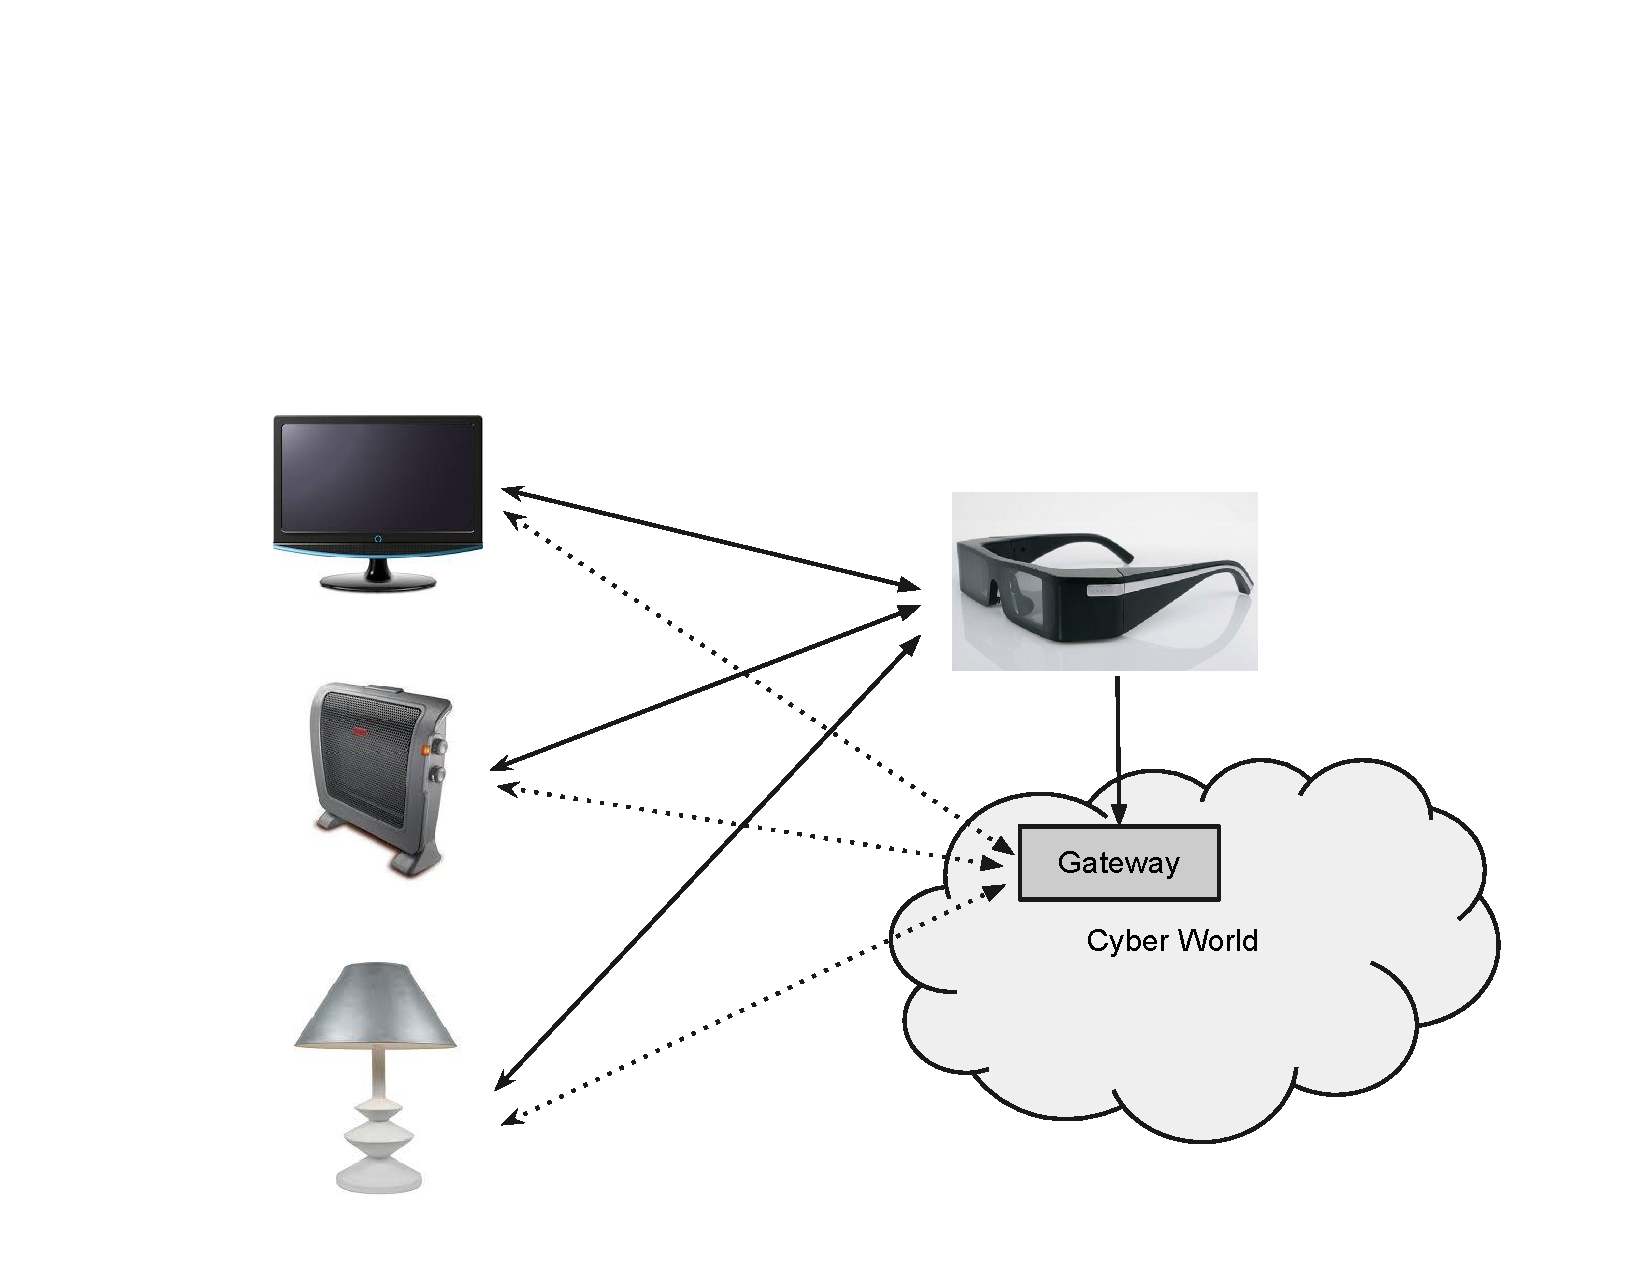
\includegraphics[width=\linewidth]{../figs/sysarch.pdf}
  \caption{System Architecture}
  \label{fig:sysarch}
\end{figure}


In our discussion, we've come up with three possible approaches. The first is a purely glass solution. The second is augmented by some computer vision detection. The third  will be a combination of glasses and smart watch. 

% Lessons learned from \cite{Bellotti:2002:MSS:503376.503450} have also guided us in thinking the Five A's when designing novel interaction system. 


%%% Local Variables: 
%%% mode: latex
%%% TeX-master: "main"
%%% End: 

